\documentclass{article}

%% Font selection
%\usepackage{lmodern}
\usepackage{bera}
%\usepackage{DejaVuSerifCondensed}
%\usepackage{beramono}
\usepackage{microtype}
\usepackage[T1]{fontenc}

%% Listings (see https://www.ctan.org/pkg/minted for installation)
\usepackage[cache=true,outputdir=.texpadtmp]{minted}
\setminted{ fontsize=\small, frame = leftline, framesep = 2\fboxsep }
\setmintedinline{ fontsize=\normalfont }
\usepackage{upquote}  % TT quotes in listings

%% Other packages
\usepackage[english]{babel}  % Language support
\usepackage{lipsum}  % TODO Remove
\usepackage{graphicx}  % Support EPS figures
\usepackage{url,hyperref}  % \url command, properly working

%% Last package of all
\usepackage{cleveref}  % Allows en­hanced cross-ref­er­enc­ing fea­tures
 
%% Shourtcuts
\usepackage{xspace}
\newcommand{\matlab}{\textsc{Matlab}\xspace}
\newcommand{\csv}{\texttt{CSV}\xspace}

%% Document details
\title{Piecewise segmentation for financial data}
\author{Paolo Antonini \and Davide Azzalini \and Fabio Azzalini}
\date{}

%% DOCUMENT
\begin{document}

\maketitle


\begin{abstract}
Time series data is characterised as large in data size, high dimensionality and update continuously. Moreover, the time series data is always considered as a whole instead of individual numerical fields. As a consequence, in order to analyse and mine time series data, segmentation and dimensionality reduction are essential. In particular, in the following pages we are going to collect and study some segmentation methods, applied in particular to stock market data. Stock time series has its own characteristics over other time series. 
\end{abstract}

\section{Introduction}
The tasks of segmentation ad dimensionality reduction are fundamental to allow many time series analysis and mining tasks. In particular, our objective is to find significant trends in stock market data, which is inherently large in size, noisy and continuously updated. 

In this paper we are going first to list some of the main research papers where dimensionality reduction and piecewise segmentation are studied, in \cref{sec:methods}. Then, in \cref{sec:implementations} we are going to present some implementations of the methods. 


\section{Methods}\label{sec:methods}
\lipsum[1-3]


\section{Implementations}\label{sec:implementations}

\lipsum[7]

\subsection{Turning points in \matlab}

Here we are presenting our implementation of the method to find \emph{turning points}, as it was presented in % TODO Where??

The method is developed and tested over \csv files downloaded from Yahoo! Finance website\footnote{\url{http://finance.yahoo.com/market-overview/}}. Should another source be used, basic adaptations may be necessary, mostly in the handling of temporal data (i.e., dates). 

After importing the aforementioned \csv file (we suggest to use the graphical interface provided by \matlab itself), the user should issue the command in \cref{lst:list1}, in order to convert dates into a tractable format, generate the matrix over which the function works and compute the results.

\begin{listing}[H]

\begin{minted}{matlab}
t = datenum(Date, 'yyyy-mm-dd');  % converts dates to tractable format
M = [t Close];  % generates the matrix
y = TurningPoints(M);  % computes the results
\end{minted}

\caption{User commands.}\label{lst:list1}

\end{listing}

%TODO Riferimento
Actually, \mintinline{matlab}{TurningPoints()} function is implemented as shown in \cref{lst:functionMatlab}. The first part of the function implements what was presented in XXX, whereas the second part performs some operations in order to present in an appropriate way the results.

\begin{listing}[H]

\inputminted{matlab}{../code/TurningPoints.m}

\caption{\texttt{TurningPoints()} function}\label{lst:functionMatlab}

\end{listing}

We also performed some tests, to guarantee the proper functioning of the implemented algorithm. Weekly stock market data from A2A (\texttt{A2A.MI}) over the whole 2015 was used as source. The result of the processing is in \cref{fig:a2a_w_2015}.

\begin{figure}
	
	\makebox[\textwidth][c]{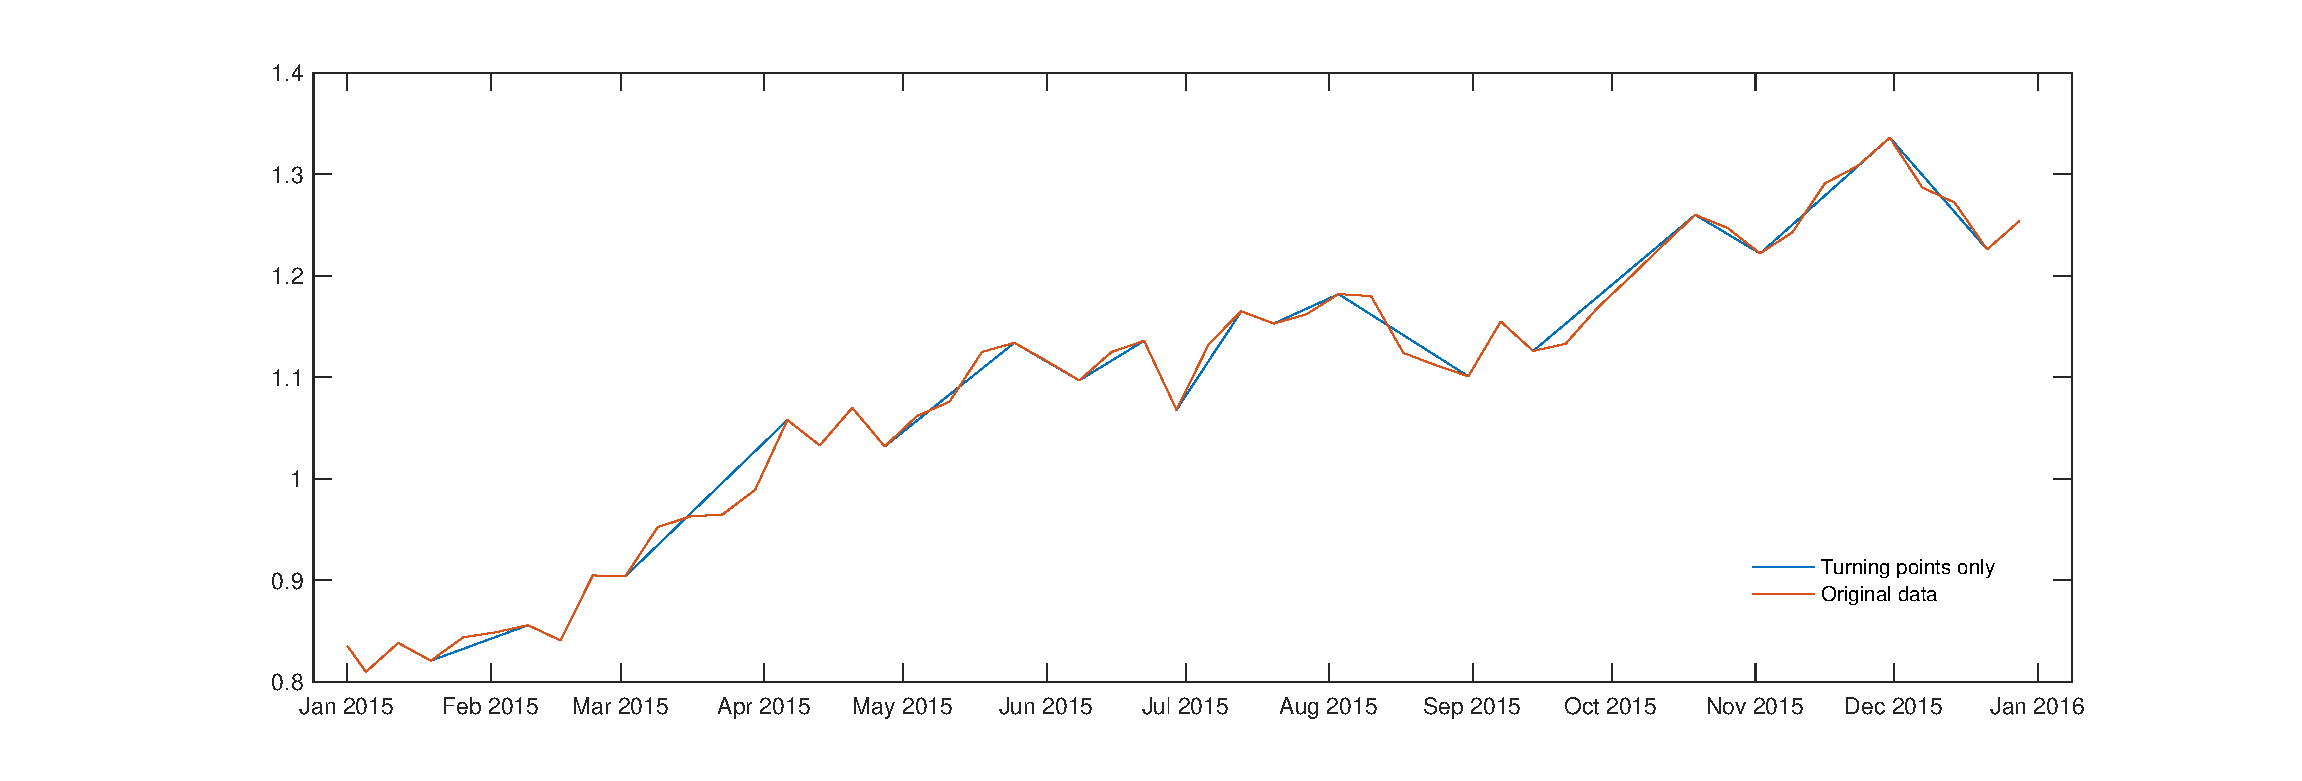
\includegraphics[width=1.8\textwidth]{img/a2a_W_15}}
	
	\caption{\texttt{A2A.MI} weekly 2015}
	
	\label{fig:a2a_w_2015}

\end{figure}



\subsection{Other implementations}
\lipsum[4-6]


\end{document}







